\documentclass[aspectratio=169,11pt]{beamer}

% ── Theme & colours ──────────────────────────────────────────────────────────
\usetheme{default}
\usecolortheme{default}
\definecolor{coral}{RGB}{205,92,70}
\definecolor{terracotta}{RGB}{178,70,45}
\definecolor{cream}{RGB}{252,248,243}
\definecolor{darkbrown}{RGB}{70,35,15}
\definecolor{lightcoral}{RGB}{245,220,210}
\definecolor{midgray}{RGB}{120,110,105}

\setbeamercolor{frametitle}{fg=terracotta,bg=cream}
\setbeamercolor{background canvas}{bg=cream}
\setbeamercolor{normal text}{fg=darkbrown}
\setbeamercolor{structure}{fg=coral}
\setbeamercolor{alerted text}{fg=terracotta}
\setbeamercolor{block title}{bg=coral,fg=white}
\setbeamercolor{block body}{bg=lightcoral!50,fg=darkbrown}
\setbeamercolor{alertblock title}{bg=terracotta,fg=white}
\setbeamercolor{itemize item}{fg=coral}
\setbeamercolor{itemize subitem}{fg=coral!70}

\setbeamertemplate{navigation symbols}{}
\setbeamertemplate{itemize item}{\textbullet}
\setbeamertemplate{itemize subitem}{--}

% Minimal footline
\setbeamertemplate{footline}{%
  \hfill\usebeamerfont{footline}%
  \textcolor{midgray}{\insertframenumber}\hspace{8pt}\vspace{4pt}%
}

% Frame title with bottom rule
\setbeamertemplate{frametitle}{%
  \vspace{8pt}%
  {\usebeamerfont{frametitle}\usebeamercolor[fg]{frametitle}\insertframetitle}%
  \vspace{2pt}\hrule height 0.4pt\relax%
  \vspace{4pt}%
}

\setbeamerfont{title}{size=\LARGE,series=\bfseries}
\setbeamerfont{subtitle}{size=\large}
\setbeamerfont{frametitle}{size=\large,series=\bfseries}
\setbeamerfont{block title}{size=\small,series=\bfseries}
\setbeamerfont{block body}{size=\small}
\setbeamerfont{footline}{size=\scriptsize}

% ── Packages ─────────────────────────────────────────────────────────────────
\usepackage[T1]{fontenc}
\usepackage[utf8]{inputenc}
\usepackage{lmodern}
\usepackage{booktabs}
\usepackage{tikz}
\usetikzlibrary{shapes,arrows.meta,positioning,calc}
\usepackage{fontawesome5}
\usepackage{xcolor}
\usepackage{array}
\usepackage{hyperref}

% ── Handy command: coloured pill tag ─────────────────────────────────────────
\newcommand{\pill}[2][coral]{%
  \tikz[baseline=-0.6ex]\node[fill=#1!15,draw=#1!40,rounded corners=3pt,
    inner xsep=5pt,inner ysep=2pt,font=\scriptsize\bfseries,text=#1]{\strut #2};%
}

% ── Metadata ─────────────────────────────────────────────────────────────────
\title{DocForge}
\subtitle{From Documents to Answers\\[4pt]
  \small Multimodal Knowledge Graph RAG for Evaluation Reports}
\author{}
\date{June 2026}
\institute{\textcolor{midgray}{Labor Innovation}}

% ─────────────────────────────────────────────────────────────────────────────
\begin{document}
% ─────────────────────────────────────────────────────────────────────────────

%%  TITLE
\begin{frame}[plain]
  \begin{center}
    \vspace{1.5cm}
    {\usebeamerfont{title}\textcolor{terracotta}{DocForge}}\\[6pt]
    {\large\textcolor{coral}{From Documents to Answers}}\\[4pt]
    {\small\textcolor{midgray}{Multimodal Knowledge Graph RAG
      for EU Evaluation Reports}}\\[1.4cm]
    {\footnotesize\textcolor{midgray}{Labor Innovation \quad|\quad June 2026}}
  \end{center}
\end{frame}

%%  AGENDA
\begin{frame}{What We Will Cover}
  \vspace{0.3cm}
  \begin{columns}[t]
    \begin{column}{0.45\textwidth}
      \begin{enumerate}\setlength\itemsep{8pt}
        \item The Problem
        \item Smart Ingestion
        \item The Knowledge Graph
        \item Answering Questions
        \item Citations \& Reasoning
      \end{enumerate}
    \end{column}
    \begin{column}{0.45\textwidth}
      \begin{enumerate}\setcounter{enumi}{5}\setlength\itemsep{8pt}
        \item How DocForge Compares
        \item Future Paths to Explore
        \item Live Demo
      \end{enumerate}
    \end{column}
  \end{columns}
\end{frame}

% ─────────────────────────────────────────────────────────────────────────────
\section{The Problem}
% ─────────────────────────────────────────────────────────────────────────────

\begin{frame}{You Have Hundreds of Reports. Now What?}
  \vspace{0.2cm}
  \begin{columns}[t]
    \begin{column}{0.55\textwidth}
      \medskip
      \begin{itemize}\setlength\itemsep{10pt}
        \item Evaluation reports are \textbf{long, complex and numerous}
        \item Key findings are buried in tables, charts and appendices
        \item Connecting insights \emph{across} programmes requires manual work
        \item Traditional search misses \textbf{meaning and context}
      \end{itemize}
    \end{column}
    \begin{column}{0.40\textwidth}
      \medskip
      \begin{block}{\small 13 reports loaded}
        \footnotesize
        POCU (3) \textbullet\ POIM \textbullet\ POR\\[3pt]
        POC \textbullet\ POCA \textbullet\ POAT\\[3pt]
        RO-BG cross-border\\[3pt]
        Themes A, C, D, E\\[3pt]
        \textcolor{midgray}{+ more as added\ldots}
      \end{block}
    \end{column}
  \end{columns}
  \vspace{0.5cm}
  \begin{center}
    \colorbox{lightcoral!60}{%
      \parbox{0.82\textwidth}{\centering\small
        Policy analysts spend \textbf{60--80\% of their time}
        \emph{locating} information rather than drawing conclusions.
      }%
    }
  \end{center}
\end{frame}

% ─────────────────────────────────────────────────────────────────────────────
\section{Smart Ingestion}
% ─────────────────────────────────────────────────────────────────────────────

\begin{frame}{Step 1 — Smart Ingestion}
  \vspace{0.1cm}
  \begin{center}
  \begin{tikzpicture}[
      node distance=1.1cm,
      box/.style={draw=coral!70,fill=lightcoral!30,rounded corners=5pt,
                  minimum width=2.3cm,minimum height=1cm,
                  align=center,font=\small\bfseries},
      arr/.style={-{Stealth},thick,coral!80}
    ]
    \node[box] (pdf)   {\faFilePdf\\[2pt]\scriptsize Your PDFs};
    \node[box,right=of pdf]  (read) {\faEye\\[2pt]\scriptsize Read\\[-1pt]\scriptsize Everything};
    \node[box,right=of read] (kg)   {\faProjectDiagram\\[2pt]\scriptsize Build\\[-1pt]\scriptsize Knowledge};
    \node[box,right=of kg]   (ans)  {\faComments\\[2pt]\scriptsize Answer\\[-1pt]\scriptsize Questions};
    \draw[arr] (pdf) -- (read);
    \draw[arr] (read) -- (kg);
    \draw[arr] (kg) -- (ans);
  \end{tikzpicture}
  \end{center}
  \bigskip
  \begin{columns}[t]
    \begin{column}{0.45\textwidth}
      \textbf{\textcolor{midgray}{What most tools do:}}\\[4pt]
      \begin{itemize}\setlength\itemsep{6pt}
        \item Extract text only
        \item Ignore charts, tables, images
        \item Lose data embedded in figures
      \end{itemize}
    \end{column}
    \begin{column}{0.50\textwidth}
      \textbf{\textcolor{coral}{What DocForge does:}}\\[4pt]
      \begin{itemize}\setlength\itemsep{6pt}
        \item Reads text, tables \emph{and} images
        \item Uses a \textbf{vision AI} to describe charts
        \item Handles Romanian \& English together
      \end{itemize}
    \end{column}
  \end{columns}
\end{frame}

\begin{frame}{Multimodal = Nothing Gets Left Behind}
  \vspace{0.3cm}
  \begin{center}
  \begin{tikzpicture}[scale=1.05]
    \node[draw=coral,fill=lightcoral!40,rounded corners=5pt,
          minimum width=3.2cm,minimum height=0.8cm,
          font=\small\bfseries] (pdf) at (0,0) {\faFilePdf\ PDF Page};

    \node[draw=coral!80,fill=lightcoral!25,rounded corners=4pt,
          minimum width=2cm,minimum height=0.7cm,font=\scriptsize,align=center]
      (t) at (-3.5,-1.8) {\faAlignLeft\\[1pt]Text};
    \node[draw=terracotta!80,fill=terracotta!10,rounded corners=4pt,
          minimum width=2cm,minimum height=0.7cm,font=\scriptsize,align=center]
      (tb) at (-1.2,-1.8) {\faTable\\[1pt]Tables};
    \node[draw=darkbrown!60,fill=darkbrown!8,rounded corners=4pt,
          minimum width=2cm,minimum height=0.7cm,font=\scriptsize,align=center]
      (ch) at (1.2,-1.8) {\faChartBar\\[1pt]Charts};
    \node[draw=coral!60,fill=lightcoral!20,rounded corners=4pt,
          minimum width=2cm,minimum height=0.7cm,font=\scriptsize,align=center]
      (im) at (3.5,-1.8) {\faImage\\[1pt]Images};

    \foreach \n in {t,tb,ch,im}
      \draw[-{Stealth},coral!60] (pdf.south) -- (\n.north);

    \node[draw=coral,fill=lightcoral!50,rounded corners=5pt,
          minimum width=7cm,minimum height=0.8cm,
          font=\small\bfseries,align=center] (out) at (0,-3.3)
          {Enriched text chunk → Knowledge Graph};

    \foreach \n in {t,tb,ch,im}
      \draw[-{Stealth},coral!60] (\n.south) -- (out.north);
  \end{tikzpicture}
  \end{center}
  \vspace{0.2cm}
  \begin{center}
    \small\textcolor{midgray}{%
      Vision AI (Gemini 2.0) describes each chart and image in words\\
      so that meaning is preserved — not just pixels.}
  \end{center}
\end{frame}

% ─────────────────────────────────────────────────────────────────────────────
\section{The Knowledge Graph}
% ─────────────────────────────────────────────────────────────────────────────

\begin{frame}{Step 2 — The Knowledge Graph}
  \vspace{0.1cm}
  \begin{columns}[c]
    \begin{column}{0.50\textwidth}
      \medskip
      \textbf{Think of it like a city map}\\[8pt]
      \begin{itemize}\setlength\itemsep{9pt}
        \item Every \textbf{programme, authority, indicator}
              is a \emph{location} on the map
        \item Every \textbf{relationship} is a \emph{road}
              connecting them
        \item You can ask: \textit{``Which roads lead\\
              from POCU to ANOFM?''}
        \item The system \textbf{follows the connections}
      \end{itemize}
      \vspace{0.5em}
      \pill{15 entity types} tailored to EU structural funds
    \end{column}
    \begin{column}{0.46\textwidth}
      \centering
      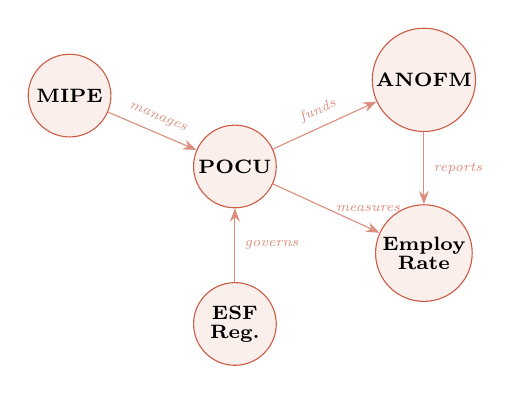
\begin{tikzpicture}[
          ent/.style={draw=coral,fill=lightcoral!45,circle,
                      minimum size=1.05cm,font=\scriptsize\bfseries,
                      align=center,inner sep=1pt},
          rel/.style={-{Stealth},coral!70,font=\scriptsize\itshape}
        ]
        \node[ent] (pocu)  at (0,0)      {POCU};
        \node[ent] (anofm) at (2.4,1.1)  {ANOFM};
        \node[ent] (mipe)  at (-2.1,0.9) {MIPE};
        \node[ent] (reg)   at (0,-2)     {ESF\\[-1pt]Reg.};
        \node[ent] (ind)   at (2.4,-1.1) {Employ\\[-1pt]Rate};
        \draw[rel] (mipe)  -- node[above,sloped]{\tiny manages} (pocu);
        \draw[rel] (pocu)  -- node[above,sloped]{\tiny funds}   (anofm);
        \draw[rel] (reg)   -- node[right]        {\tiny governs} (pocu);
        \draw[rel] (pocu)  -- node[right]        {\tiny measures}(ind);
        \draw[rel] (anofm) -- node[right]        {\tiny reports} (ind);
      \end{tikzpicture}
    \end{column}
  \end{columns}
\end{frame}

\begin{frame}{Why a Graph Changes Everything}
  \vspace{0.2cm}
  \begin{columns}[t]
    \begin{column}{0.46\textwidth}
      \textbf{\textcolor{midgray}{Without a graph}}\\[6pt]
      \begin{itemize}\setlength\itemsep{8pt}
        \item Finds pages \emph{containing} your words
        \item Cannot follow relationships
        \item Cannot compare across programmes
        \item Returns isolated snippets
      \end{itemize}
    \end{column}
    \hfill\vrule\hfill
    \begin{column}{0.46\textwidth}
      \textbf{\textcolor{coral}{With DocForge's graph}}\\[6pt]
      \begin{itemize}\setlength\itemsep{8pt}
        \item Understands that POCU \emph{relates to} ANOFM
        \item Answers: ``Which programmes share the same indicator?''
        \item Synthesises across \textbf{all 13 reports}
        \item Answers with \textbf{traceable reasoning}
      \end{itemize}
    \end{column}
  \end{columns}
  \vspace{0.7cm}
  \begin{center}
    \colorbox{lightcoral!60}{%
      \parbox{0.82\textwidth}{\centering\small
        The graph stores \textbf{entities + relationships + summaries}
        from all reports simultaneously — and stays up to date as
        new documents are added.
      }%
    }
  \end{center}
\end{frame}

% ─────────────────────────────────────────────────────────────────────────────
\section{Answering Questions}
% ─────────────────────────────────────────────────────────────────────────────

\begin{frame}{Step 3 — Ask in Plain Language}
  \vspace{0.2cm}
  \begin{columns}[t]
    \begin{column}{0.50\textwidth}
      \textbf{Example questions}\\[8pt]
      \begin{itemize}\setlength\itemsep{10pt}
        \item \textit{``What were the main barriers\\
              to POCU implementation?''}
        \item \textit{``Which programmes showed\\
              the best employment outcomes?''}
        \item \textit{``What monitoring weaknesses\\
              appear across all programmes?''}
        \item \textit{``Compare POIM and POR\\
              financial absorption rates.''}
      \end{itemize}
    \end{column}
    \begin{column}{0.46\textwidth}
      \begin{block}{Five retrieval strategies}
        \begin{description}[\textbf{Hybrid}]\setlength\itemsep{5pt}
          \item[\textbf{Local}] Deep dive on specific entities
          \item[\textbf{Global}] Themes across all documents
          \item[\textbf{Hybrid}] Local + Global combined
          \item[\textbf{Mix}] Graph + direct text search
          \item[\textbf{Naive}] Fast keyword-style search
        \end{description}
      \end{block}
      \vspace{0.3em}
      {\scriptsize Type \texttt{/global} or \texttt{/local} before your question
       to pick the strategy.}
    \end{column}
  \end{columns}
\end{frame}

% ─────────────────────────────────────────────────────────────────────────────
\section{Citations \& Reasoning}
% ─────────────────────────────────────────────────────────────────────────────

\begin{frame}{Citations \& Reasoning — Why They Matter}
  \vspace{0.2cm}
  \begin{columns}[t]
    \begin{column}{0.50\textwidth}
      \begin{itemize}\setlength\itemsep{10pt}
        \item AI systems can \textbf{confabulate} — produce
              plausible but false information
        \item Every DocForge claim is linked to the
              \textbf{exact document and section}
        \item Evaluators can \textbf{verify} any statement
              in seconds
        \item No more ``the AI said so'' without proof
      \end{itemize}
      \vspace{0.6em}
      \colorbox{lightcoral!60}{%
        \parbox{0.9\linewidth}{\scriptsize\centering
          Graph RAG reduces hallucinations by up to
          \textbf{73\%} vs.\ standard AI models.
        }%
      }
    \end{column}
    \begin{column}{0.46\textwidth}
      \begin{block}{Example cited answer}
        \small
        POCU faced significant administrative
        capacity issues including recruitment
        bottlenecks \textcolor{coral}{[1]}
        and communication gaps \textcolor{coral}{[2]}.
      \end{block}
      \vspace{0.5em}
      \begin{alertblock}{Sources}
        \small
        \textcolor{white}{[1]}\ 01\_POCU\_Education.pdf\\[2pt]
        \textcolor{white}{[2]}\ 07\_POCU\_Ocupare.pdf
      \end{alertblock}
      \vspace{0.4em}
      {\scriptsize\itshape\textcolor{midgray}{%
        Click any source to read the original passage.}}
    \end{column}
  \end{columns}
  \vspace{0.5em}
  \begin{center}
    \colorbox{lightcoral!60}{%
      \parbox{0.88\textwidth}{\centering\small
        \textbf{Citations} give you proof — trace every claim back to its source.
        The \textbf{Reasoning panel} gives you insight — it connects dots across
        all 13 reports at once, something that would take a human analyst days.
      }%
    }
  \end{center}
\end{frame}

\begin{frame}{AI Reasoning: The ``Why'' Behind the Answer}
  \vspace{0.2cm}
  \begin{columns}[t]
    \begin{column}{0.48\textwidth}
      \textbf{Standard answer}\\[6pt]
      \begin{quote}\small\itshape
        ``POCU faced challenges: recruitment
         delays, limited procurement capacity
         and communication gaps.''
      \end{quote}
      \vspace{0.6em}
      \textbf{DocForge Synthesis adds}\\[6pt]
      \begin{quote}\small\itshape
        ``The \textbf{same administrative weaknesses}
         appear in POIM, POR and POCA — suggesting
         a \textbf{systemic structural issue}
         across all managing authorities,
         not a POCU-specific problem.''
      \end{quote}
    \end{column}
    \begin{column}{0.48\textwidth}
      \begin{block}{What the Synthesis panel does}
        \begin{itemize}\setlength\itemsep{7pt}
          \item A \textbf{second AI analysis} runs on
                the retrieved knowledge graph
          \item Surfaces \textbf{patterns and\\
                cross-programme connections}
          \item Separates \emph{what documents say}
                from \emph{what the graph implies}
          \item Always shown separately from the answer
        \end{itemize}
      \end{block}
    \end{column}
  \end{columns}
\end{frame}

\begin{frame}{Custom Instructions — Tailoring Every Answer}
  \vspace{0.3cm}
  \begin{center}
    \small Type a one-line instruction once.
    It applies to \textbf{every query} in the session.
  \end{center}
  \bigskip
  \begin{columns}[t]
    \begin{column}{0.48\textwidth}
      \textbf{Useful examples}\\[8pt]
      \begin{itemize}\setlength\itemsep{8pt}
        \item \texttt{Answer in Romanian.}
        \item \texttt{Keep answers under 150 words.}
        \item \texttt{Include budget figures when available.}
        \item \texttt{Answer as a senior EU evaluator.}
      \end{itemize}
    \end{column}
    \begin{column}{0.46\textwidth}
      \begin{block}{Multilingual knowledge base}
        \begin{itemize}\setlength\itemsep{7pt}
          \item Romanian \& English documents
                live in the \textbf{same graph}
          \item Set \texttt{Answer in Romanian.}
                to receive all responses in Romanian
          \item Source citations always show the
                original document language
        \end{itemize}
      \end{block}
    \end{column}
  \end{columns}
\end{frame}

% ─────────────────────────────────────────────────────────────────────────────
\section{How DocForge Compares}
% ─────────────────────────────────────────────────────────────────────────────

\begin{frame}{Where DocForge Sits in the Landscape}
  \vspace{0.2cm}
  \begin{center}
  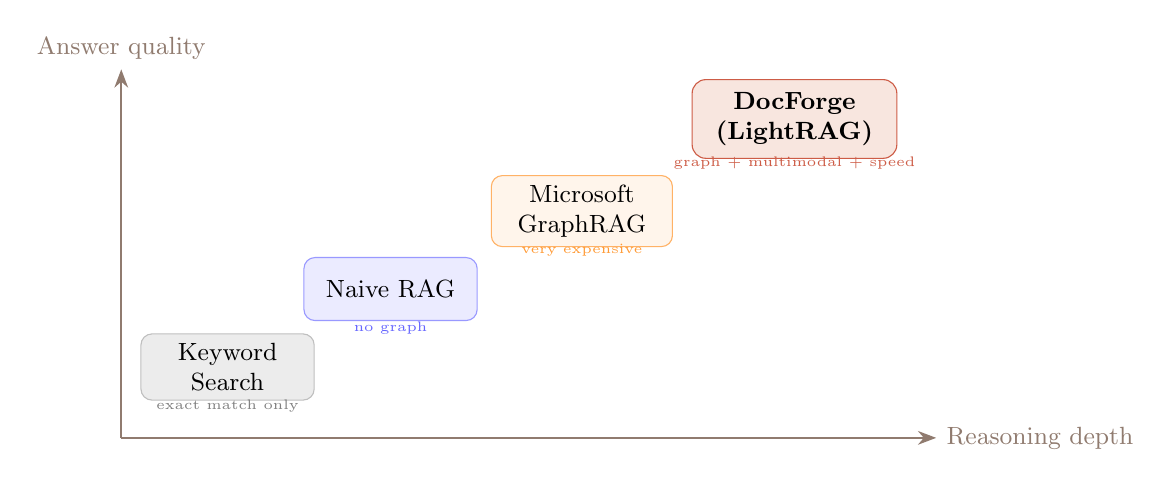
\begin{tikzpicture}[scale=0.9]
    \draw[-{Stealth},thick,darkbrown!60] (0,0) -- (11.5,0)
      node[right,font=\small] {Reasoning depth};
    \draw[-{Stealth},thick,darkbrown!60] (0,0) -- (0,5.2)
      node[above,font=\small] {Answer quality};

    \node[draw=gray!50,fill=gray!15,rounded corners=4pt,
          minimum width=2.2cm,minimum height=0.8cm,
          font=\small,align=center] at (1.5,1.0) {Keyword\\Search};
    \node[font=\tiny,text=gray] at (1.5,0.45) {exact match only};

    \node[draw=blue!40,fill=blue!8,rounded corners=4pt,
          minimum width=2.2cm,minimum height=0.8cm,
          font=\small,align=center] at (3.8,2.1) {Naive RAG};
    \node[font=\tiny,text=blue!60] at (3.8,1.55) {no graph};

    \node[draw=orange!60,fill=orange!8,rounded corners=4pt,
          minimum width=2.3cm,minimum height=0.8cm,
          font=\small,align=center] at (6.5,3.2) {Microsoft\\GraphRAG};
    \node[font=\tiny,text=orange!80] at (6.5,2.65) {very expensive};

    \node[draw=coral,fill=lightcoral!70,rounded corners=5pt,
          minimum width=2.6cm,minimum height=1.0cm,
          font=\small\bfseries,align=center] at (9.5,4.5) {DocForge\\(LightRAG)};
    \node[font=\tiny,text=coral] at (9.5,3.88) {graph + multimodal + speed};
  \end{tikzpicture}
  \end{center}
\end{frame}

\begin{frame}{Head-to-Head Comparison}
  \vspace{0.2cm}
  \centering
  \renewcommand{\arraystretch}{1.4}
  \begin{tabular}{lcccc}
    \toprule
    \textbf{Capability} &
    \textbf{Keyword} &
    \textbf{Naive RAG} &
    \textbf{GraphRAG} &
    \textbf{DocForge} \\
    \midrule
    Reads tables \& charts
      & \textcolor{gray}{\faTimes}
      & \textcolor{gray}{\faTimes}
      & \textcolor{gray}{\faTimes}
      & \textcolor{coral}{\faCheck} \\
    Cross-document reasoning
      & \textcolor{gray}{\faTimes}
      & \textcolor{gray!60}{$\sim$}
      & \textcolor{coral}{\faCheck}
      & \textcolor{coral}{\faCheck} \\
    Knowledge graph
      & \textcolor{gray}{\faTimes}
      & \textcolor{gray}{\faTimes}
      & \textcolor{coral}{\faCheck}
      & \textcolor{coral}{\faCheck} \\
    Cited answers
      & \textcolor{gray}{\faTimes}
      & \textcolor{gray!60}{$\sim$}
      & \textcolor{coral}{\faCheck}
      & \textcolor{coral}{\faCheck} \\
    AI Synthesis / reasoning
      & \textcolor{gray}{\faTimes}
      & \textcolor{gray}{\faTimes}
      & \textcolor{coral}{\faCheck}
      & \textcolor{coral}{\faCheck} \\
    Fast \& affordable
      & \textcolor{coral}{\faCheck}
      & \textcolor{coral}{\faCheck}
      & \textcolor{gray}{\faTimes}
      & \textcolor{coral}{\faCheck} \\
    Romanian language
      & \textcolor{gray}{\faTimes}
      & \textcolor{gray!60}{$\sim$}
      & \textcolor{gray!60}{$\sim$}
      & \textcolor{coral}{\faCheck} \\
    \bottomrule
  \end{tabular}
  \vspace{0.5em}\\
  {\scriptsize GraphRAG sends the \textbf{entire corpus} to the LLM per query (500k+ tokens).
   LightRAG retrieves only what is relevant (10--30k tokens) — a \textbf{20--50$\times$ cost reduction}
   with comparable answer quality.}
\end{frame}

\begin{frame}{What the Research Shows}
  \vspace{0.3cm}
  \begin{columns}[t]
    \begin{column}{0.46\textwidth}
      \begin{block}{LightRAG benchmarks}
        \begin{itemize}\setlength\itemsep{7pt}
          \item \textbf{80\%+} retrieval accuracy on policy docs\\
                vs.\ 60--70\% for other methods
          \item Outperforms Naive RAG, GraphRAG, HyDE
                on all four quality dimensions
          \item \textbf{20--30 ms} faster responses than
                standard graph RAG
        \end{itemize}
      \end{block}
    \end{column}
    \begin{column}{0.46\textwidth}
      \begin{block}{Hallucination \& multimodal}
        \begin{itemize}\setlength\itemsep{7pt}
          \item Graph grounding reduces hallucinations
                by \textbf{73\%} vs.\ standard LLMs
          \item Multimodal RAG reached \textbf{enterprise
                maturity in 2026} — first viable year for
                production PDF pipelines with vision
          \item Vision models preserve data hidden in
                charts that text-only tools miss
        \end{itemize}
      \end{block}
    \end{column}
  \end{columns}
\end{frame}

% ─────────────────────────────────────────────────────────────────────────────
\section{Future Paths to Explore}
% ─────────────────────────────────────────────────────────────────────────────

\begin{frame}{Where the Field Is Heading}
  \vspace{0.2cm}
  \begin{columns}[t]
    \begin{column}{0.46\textwidth}
      \begin{block}{\faRobot\ Agentic RAG}
        \begin{itemize}\setlength\itemsep{6pt}
          \item The AI \textbf{plans its own search}:
                decomposes complex questions, retrieves
                iteratively and checks its own answers
          \item Like hiring a research assistant instead
                of asking a librarian for one book
          \item Enables 3--5 step reasoning chains across
                multiple programmes
        \end{itemize}
      \end{block}
    \end{column}
    \begin{column}{0.46\textwidth}
      \begin{block}{\faSync\ Corrective RAG (CRAG)}
        \begin{itemize}\setlength\itemsep{6pt}
          \item After retrieval, the system
                \textbf{grades its own evidence}
          \item If evidence is weak, it re-queries
                automatically
          \item Reduces hallucinations by a further
                \textbf{20--40\%} on complex queries
          \item Signals low-confidence answers rather
                than generating unsupported text
        \end{itemize}
      \end{block}
    \end{column}
  \end{columns}
\end{frame}

\begin{frame}{More Paths Worth Exploring — Routing \& Fine-Tuning}
  \vspace{0.2cm}
  \begin{columns}[t]
    \begin{column}{0.46\textwidth}
      \begin{block}{\faRoute\ Adaptive Retrieval Routing}
        \begin{itemize}\setlength\itemsep{8pt}
          \item A classifier \textbf{automatically picks}
                the best mode per question
          \item Simple question → fast naive search
          \item Cross-programme theme → global graph
          \item Complex multi-step → agentic reasoning
        \end{itemize}
      \end{block}
    \end{column}
    \begin{column}{0.46\textwidth}
      \begin{block}{\faMicrochip\ Domain Embedding Fine-Tuning}
        \begin{itemize}\setlength\itemsep{8pt}
          \item Train embeddings specifically on EU
                structural fund vocabulary
          \item Terms like ``absorption rate'' and
                ``managing authority'' cluster correctly
                from day one
          \item Improves search quality for all
                retrieval modes
        \end{itemize}
      \end{block}
    \end{column}
  \end{columns}
\end{frame}

\begin{frame}{More Paths Worth Exploring — Quality \& Currency}
  \vspace{0.2cm}
  \begin{columns}[t]
    \begin{column}{0.46\textwidth}
      \begin{block}{\faChartBar\ Automated Quality Testing}
        \begin{itemize}\setlength\itemsep{8pt}
          \item Run a golden test set of known questions
                \textbf{after every new document} is added
          \item Detect regressions in answer quality
                automatically — like unit tests for knowledge
          \item DocForge already has a RAGAS evaluation
                tab; next step is scheduling it
        \end{itemize}
      \end{block}
    \end{column}
    \begin{column}{0.46\textwidth}
      \begin{block}{\faGlobe\ Real-Time Web Retrieval}
        \begin{itemize}\setlength\itemsep{8pt}
          \item Pull current regulations or news
                alongside the document corpus
          \item Useful when regulations change
                after the reports were written
          \item Hybrid retrieval: local knowledge graph
                + live web search in one answer
        \end{itemize}
      \end{block}
    \end{column}
  \end{columns}
\end{frame}

\begin{frame}{Opportunity Map}
  \vspace{0.1cm}
  \centering
  \renewcommand{\arraystretch}{1.45}
  \begin{tabular}{p{4cm}ccp{3.8cm}}
    \toprule
    \textbf{Enhancement} &
    \textbf{Impact} &
    \textbf{Effort} &
    \textbf{Best for} \\
    \midrule
    Corrective RAG (CRAG)      & \textcolor{coral}{High}   & Low    & Reducing silent errors \\
    Adaptive routing           & \textcolor{coral}{High}   & Low    & Ease of use \\
    Automated RAGAS benchmarks & Medium & Low    & Quality monitoring \\
    Domain embedding fine-tune & \textcolor{coral}{High}   & Medium & EU/policy vocabulary \\
    Incremental graph updates  & Medium & Medium & Growing corpora \\
    Agentic multi-hop RAG      & \textcolor{coral}{Very High} & High & Complex evaluations \\
    Real-time web retrieval    & Medium & Medium & Current regulations \\
    \bottomrule
  \end{tabular}
  \vspace{0.5em}
  \begin{center}
    \colorbox{lightcoral!60}{%
      \parbox{0.82\textwidth}{\centering\small
        \textbf{Recommended first step:}
        Corrective RAG + Adaptive routing —
        high impact, low effort, no change to the user experience.
      }%
    }
  \end{center}
\end{frame}

% ─────────────────────────────────────────────────────────────────────────────
\section{Live Demo}
% ─────────────────────────────────────────────────────────────────────────────

\begin{frame}{The DocForge Interface}
  \vspace{0.1cm}
  \begin{columns}[t]
    \begin{column}{0.48\textwidth}
      \textbf{Left — Chat}
      \begin{itemize}\setlength\itemsep{7pt}
        \item Type any question in plain language
        \item Answers arrive with cited sources
        \item Full conversation history
        \item Click a past question to reload insights
      \end{itemize}
      \vspace{0.5em}
      \textbf{Right — Insights panel}
      \begin{itemize}\setlength\itemsep{7pt}
        \item \textit{AI Reasoning} — synthesis over the graph
        \item \textit{Entities \& Relationships} retrieved
        \item \textit{Sources} — exact text passages used
      \end{itemize}
    \end{column}
    \begin{column}{0.48\textwidth}
      \begin{block}{Settings}
        \begin{itemize}\setlength\itemsep{6pt}
          \item Choose retrieval mode
          \item Add custom instructions
          \item Adjust how much of the graph to use
        \end{itemize}
      \end{block}
      \vspace{0.5em}
      \begin{alertblock}{Currently loaded}
        \textbf{13 EU/Romania evaluation reports}\\[4pt]
        POCU · POIM · POR · POC · POCA · POAT\\
        RO-BG cross-border · Themes A, C, D, E
      \end{alertblock}
    \end{column}
  \end{columns}
\end{frame}

\begin{frame}{Try These Questions Now}
  \vspace{0.3cm}
  \begin{enumerate}\setlength\itemsep{14pt}
    \item \textit{``What were the main barriers to implementation\\
          across all operational programmes?''}\\
          {\small\textcolor{midgray}{\texttt{/global} — synthesises themes across all 13 reports}}

    \item \textit{``What specific employment targets did POCU set\\
          and were they achieved?''}\\
          {\small\textcolor{midgray}{\texttt{/local} — retrieves precise indicator data}}

    \item \textit{``Compare the monitoring weaknesses identified\\
          in POIM and POR.''}\\
          {\small\textcolor{midgray}{\texttt{/hybrid} — cross-programme comparison}}

    \item \textit{``Care sunt principalele recomandări pentru\\
          îmbunătățirea absorbției fondurilor?''}\\
          {\small\textcolor{midgray}{Romanian question, set custom prompt: \texttt{Answer in Romanian.}}}
  \end{enumerate}
\end{frame}

% ─────────────────────────────────────────────────────────────────────────────
%  Summary
% ─────────────────────────────────────────────────────────────────────────────

\begin{frame}{Summary}
  \vspace{0.2cm}
  \begin{columns}[t]
    \begin{column}{0.50\textwidth}
      \textbf{DocForge gives you:}\\[8pt]
      \begin{enumerate}\setlength\itemsep{9pt}
        \item \textbf{Complete ingestion} — text, tables, charts, images
        \item \textbf{Knowledge graph} — permanent map of all findings
        \item \textbf{Plain-language Q\&A} — cited, verifiable answers
        \item \textbf{AI Synthesis} — surfaces systemic patterns
        \item \textbf{Multilingual} — Romanian + English in one base
      \end{enumerate}
    \end{column}
    \begin{column}{0.46\textwidth}
      \begin{alertblock}{\faGlobe\ Try it now}
        \centering\medskip
        \textbf{docforge.labor-innovation.com}\\[6pt]
        {\small No login required.\\
         13 reports already loaded.}
        \medskip
      \end{alertblock}
      \vspace{0.5em}
      \begin{block}{Under the hood}
        {\small
         LightRAG · Claude Sonnet · Gemini 2.0\\
         Docker · Dokploy · OpenRouter}
      \end{block}
    \end{column}
  \end{columns}
\end{frame}

% ─────────────────────────────────────────────────────────────────────────────
%  References
% ─────────────────────────────────────────────────────────────────────────────

\begin{frame}[allowframebreaks]{References}
  \begin{thebibliography}{9}\footnotesize
    \bibitem{lightrag}
      Guo et al.\ (2024). \textit{LightRAG: Simple and Fast RAG}.
      \url{https://arxiv.org/abs/2410.05779}

    \bibitem{graphrag}
      Maarga Systems (2025). \textit{GraphRAG vs.\ LightRAG}.
      \url{https://www.maargasystems.com/2025/05/12/understanding-graphrag-vs-lightrag}

    \bibitem{ragkgil}
      RAG-KG-IL (2025). \textit{Reducing Hallucinations via KG Integration}.
      arXiv:2503.13514.

    \bibitem{multimodal}
      Zimmermann (2026). \textit{Multimodal RAG 2026: State of the Art}.
      \url{https://helain-zimmermann.com/blog/multimodal-rag-2026}

    \bibitem{crag}
      Yan et al.\ (2024). \textit{Corrective Retrieval Augmented Generation}.
      \url{https://arxiv.org/abs/2401.15884}

    \bibitem{agentic}
      MarsDevs (2026). \textit{Agentic RAG: The 2026 Production Guide}.
      \url{https://www.marsdevs.com/guides/agentic-rag-2026-guide}

    \bibitem{graphraft}
      GraphRAFT (2025). \textit{Retrieval Augmented Fine-Tuning for KGs}.
      arXiv:2504.05478.
  \end{thebibliography}
\end{frame}

\end{document}
